%---------------------------------------------------------------------

\section{MVP}
\subsection*{MVP}

%---------------------------------------------------------------------
% \SubItem{Perfis de Usuário}
% 	        \SubItem{Arquitetura}
% 	        \SubItem{Licença}
% 	        \SubItem{DevOps}
%######################################################################
\begin{frame}{{\sffamily Análise e Projeto do MVP}}
\begin{block}{Perfis de Usuário}
    \begin{itemize}
        \item Participante
        \item Instrutor
        \item Proponente
        \item Coordenador
        \item Supervisor
        
        \item Participante Externo
    \end{itemize}
\end{block}
\end{frame}
%######################################################################}

%######################################################################
\begin{frame}{{\sffamily Casos de Uso}}
    \begin{figure}
        \vfill
        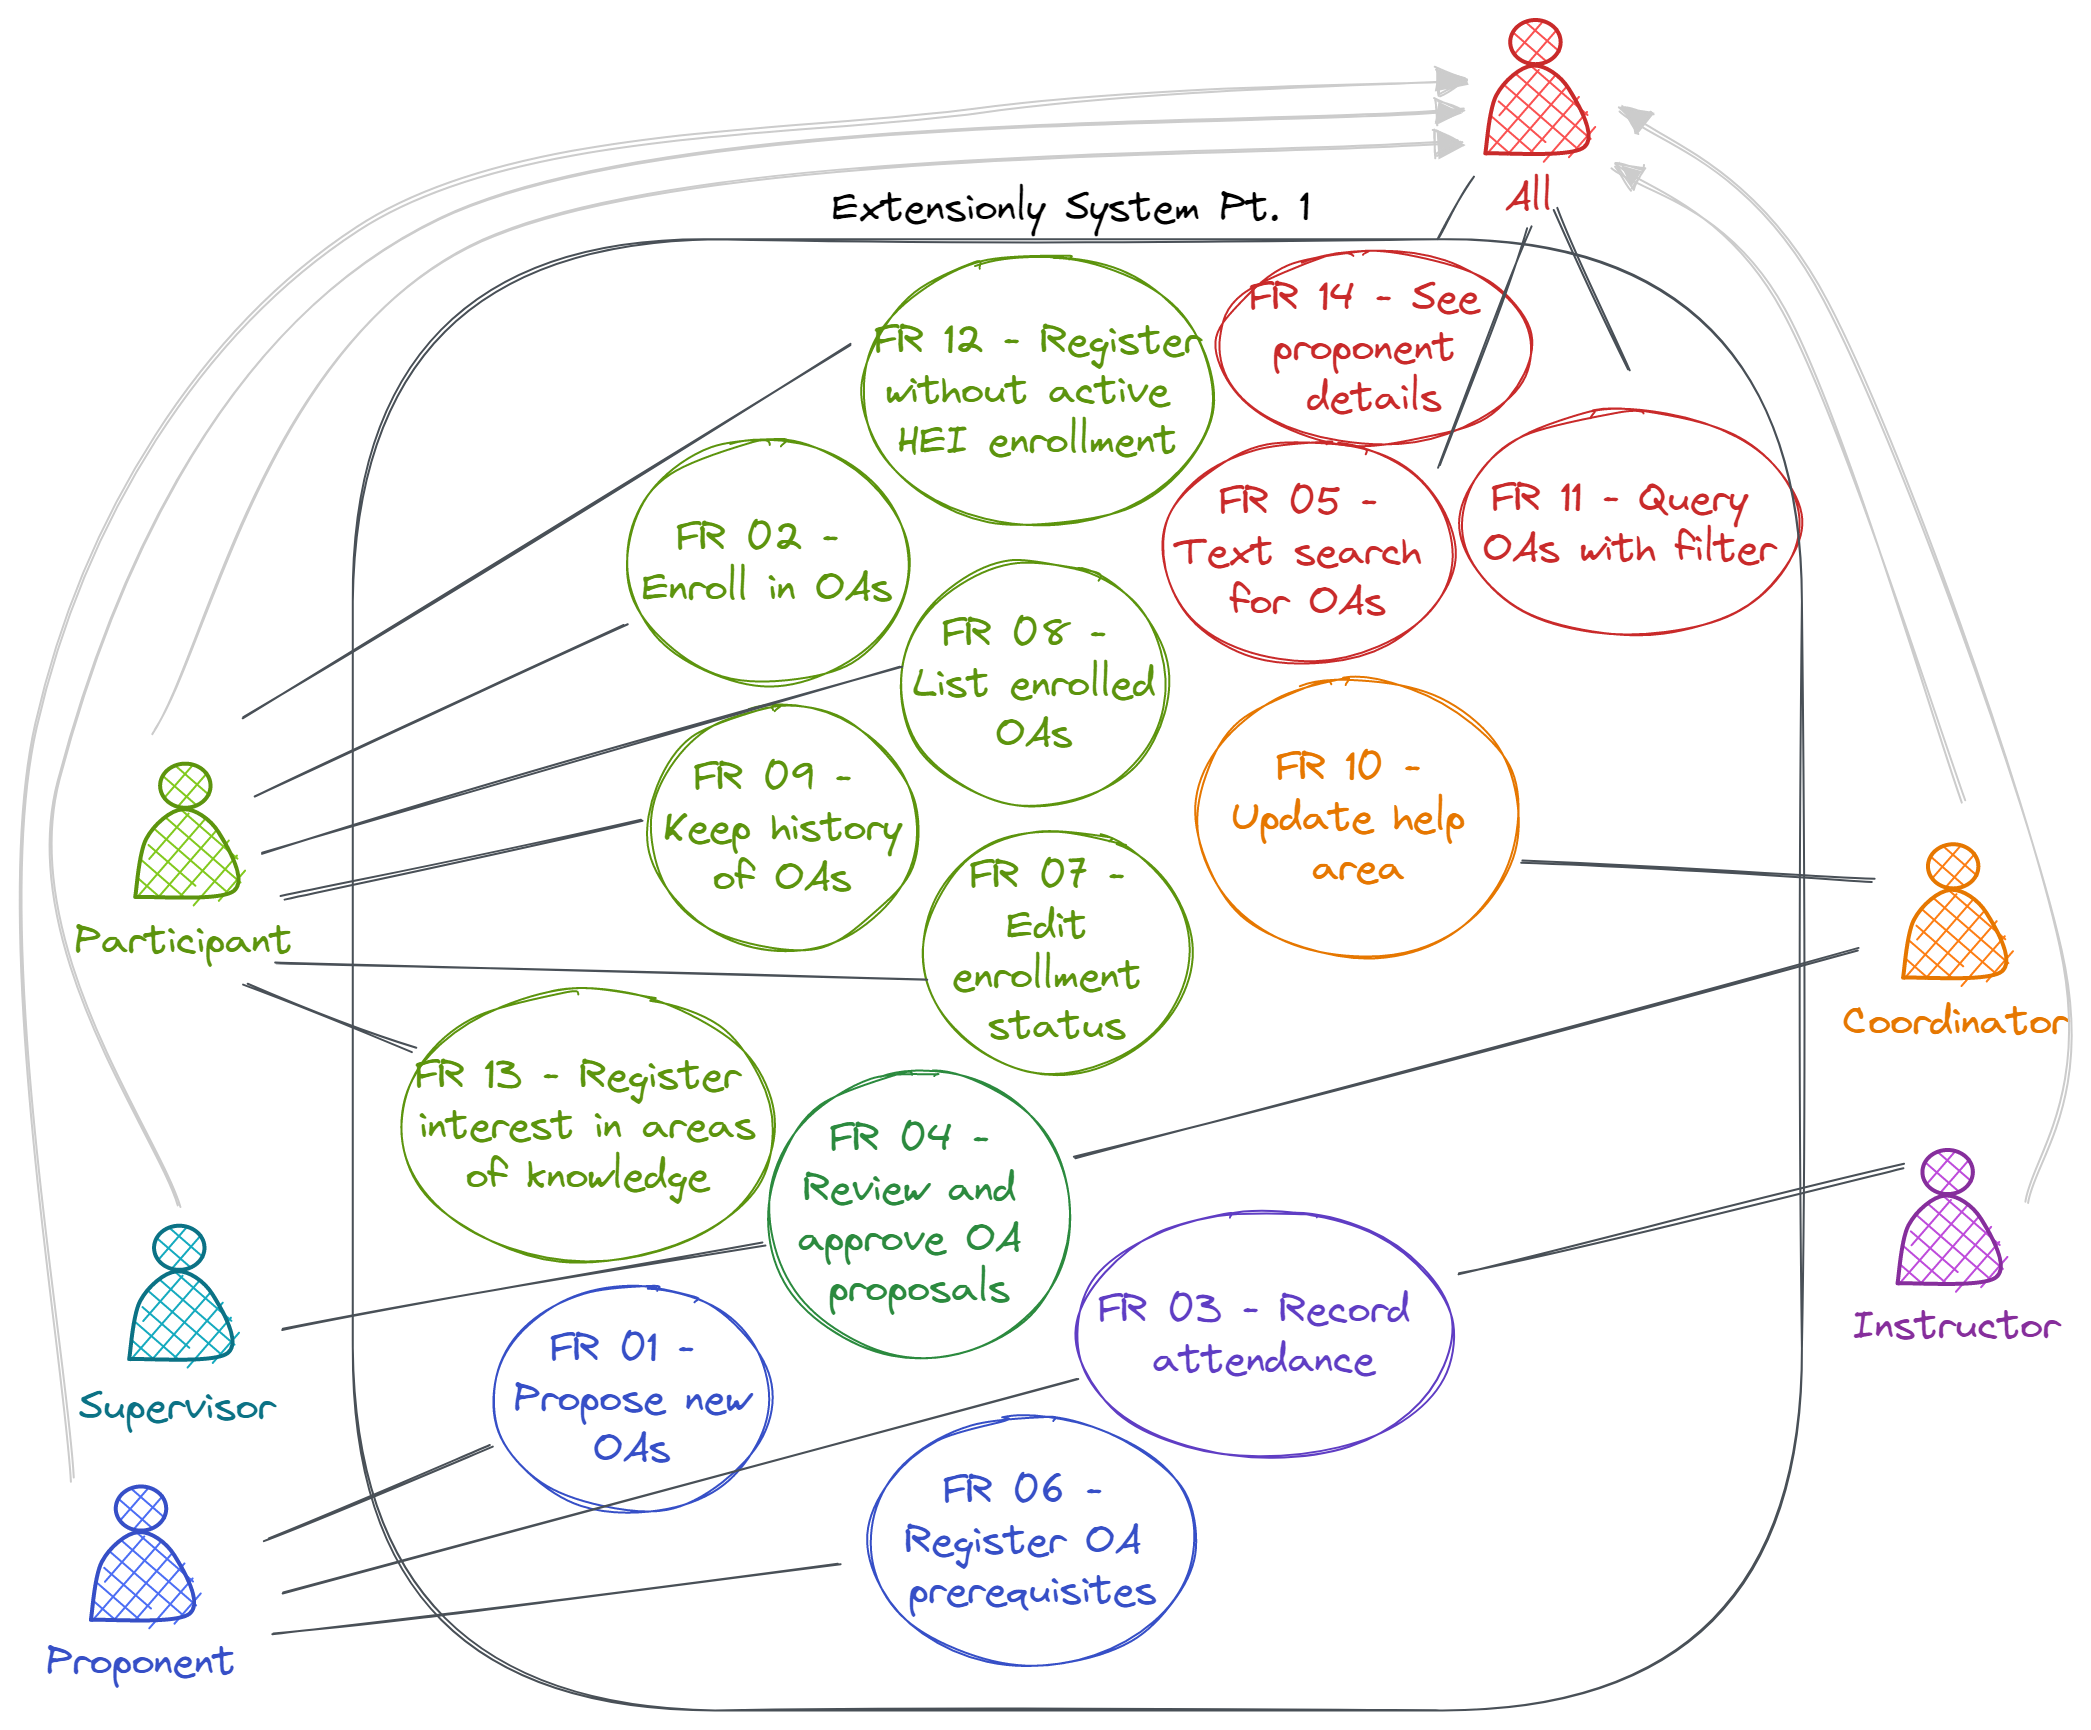
\includegraphics[width=7.5cm, ]{imagens/6-use-case-1.png}
        \vfill
    \end{figure}
\end{frame}
%######################################################################}

%######################################################################
\begin{frame}{{\sffamily Casos de Uso}}
    \begin{figure}
        \vfill
        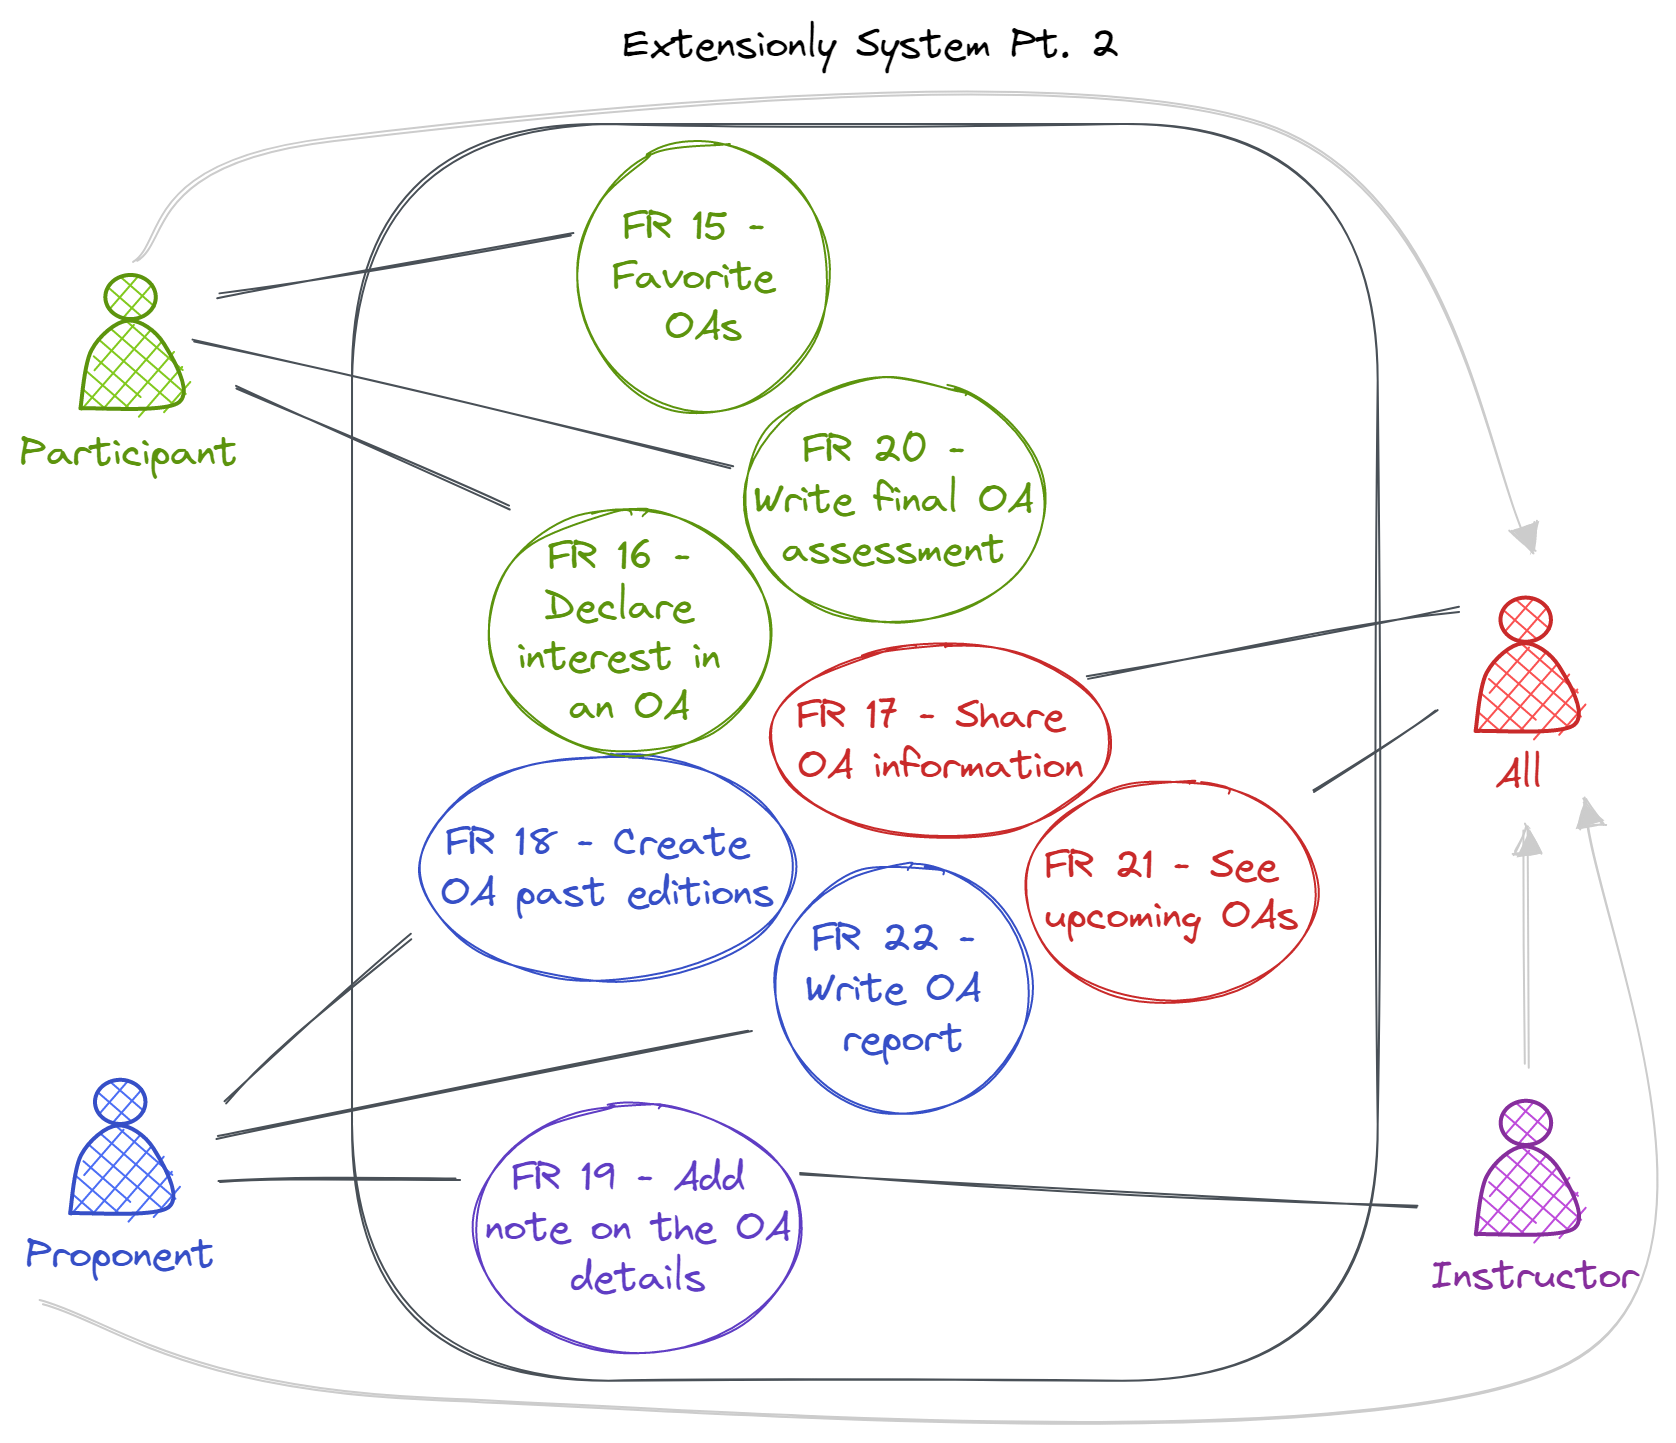
\includegraphics[width=7.5cm, ]{imagens/6-use-case-2.png}
        \vfill
    \end{figure}
\end{frame}
%######################################################################}

%######################################################################
\begin{frame}{{\sffamily Análise e Projeto do MVP}}
\begin{block}{Decisões de Projeto}
    \begin{itemize}
        \item Linguagem de programação: 
            \SubItem{TypeScript}
        \item Framework: 
            \SubItem{NestJs}
        \item Arquitetura: 
            \SubItem{Cliente-Servidor}
        \item Persistência de dados:
            \SubItem{MySQL}
            \SubItem{Prisma (ORM)}
    \end{itemize}
\end{block}
\end{frame}
%######################################################################}

%######################################################################
\begin{frame}{{\sffamily Arquitetura}}
% % \frame[allowpagebreak,T]
% % {%
%         \only<1>
%         {%
%             \centering
%             \vfill
%             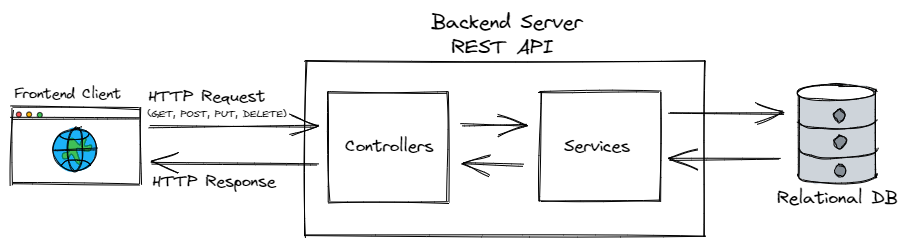
\includegraphics[height=2cm\textheight-0.5in]{imagens/6-architecture.png}
%         }%
% % }
    \begin{figure}
        \vfill
        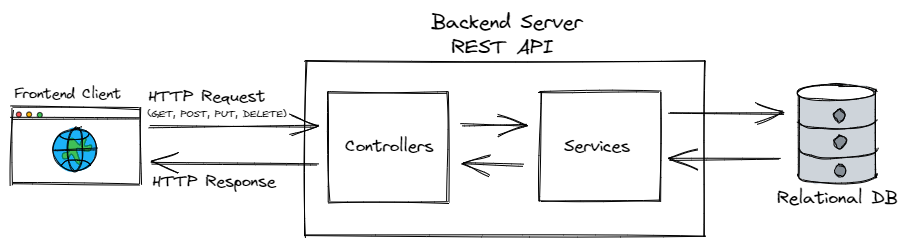
\includegraphics[width=10.5cm, ]{imagens/6-architecture.png}
        \vfill
    \end{figure}

\end{frame}
%######################################################################}

%######################################################################
\begin{frame}{{\sffamily DevOps}}
\begin{block}{DevOps}
    \begin{itemize}
        \item Integração Contínua (CI):
            \SubItem{Divisão de branches}
            \SubItem{Pipelines para testes automatizados}
        \item Entrega Contínua (CDE):
            \SubItem{Versionamento por tags}
            \SubItem{Pipelines para deploy}
        \item Solução PaaS do Heroku
    \end{itemize}
\end{block}
\end{frame}
%######################################################################}